\subsection{齐性空间与商群}

命题 11. 设 \(\mathbf{X}\) 为李群，\(\mathbf{G}\) 为 \(\mathbf{X}\) 的李子群。

\begin{enumerate}
\def\labelenumi{(\roman{enumi})}
\item
  齐性集 X/G 上存在唯一的解析流形结构，使从 X 到 X/G 的典范投影 \(\pi\) 是浸没。X 在 X/G 上的作用律是解析的。对于所有 \(x \in X\)，\(\mathrm{T}_{x}(\pi)\) 的核由 \(\mathrm{T}_{e}(\mathrm{G})\) 经 \(\mathrm{T}_{e}(\gamma(x))\) 得到。
\item
  如果 \(\mathbf{G}\) 是 \(\mathbf{X}\) 的正规子群，则 \(\mathbf{X} / \mathbf{G}\) 配以其群结构和 (i) 中定义的流形结构后是李群。映射 \(\pi\) 是李群态射。
\end{enumerate}

由 General Topology, Chapter III, § 4, no. 1, Example 1，G 通过右平移在 X 上适当且自由地作用。因此 (i) 的第一个断言由

第 5 号中的命题 10 得出。第二个断言由第 5 号的备注得出。由于 \(\pi\) 是浸没，\(T_{x}(\pi)\) 的核是 \(x\) 处下列集合的切空间：

\[
\pi^ {- 1} (\pi (x)) = x \mathrm{G} = \gamma (x) (\mathrm{G})
\]

因而它由 \(T_{e}(G)\) 经 \(T_{e}(\gamma(x))\) 得到。

设 G 是正规的。令 \(m\) 为映射 \((x,y)\mapsto xy^{-1}\)，它从 \((\mathrm{X / G})\times (\mathrm{X / G})\) 到 X/G。于是 \((m\circ (\pi \times \pi))(x,y) = \pi (xy^{-1})\) 对 X 中所有 \(x,y\) 成立。因此 \(m\circ (\pi \times \pi)\) 是解析的。由于 \(\pi \times \pi\) 是满射浸没，\(m\) 是解析的（Differentiable and Analytic Manifolds, R. 5.9.5），从而得到 (ii)。

带有 (i) 中定义的流形结构的齐性集 X/G 称为 X 关于 G 的商（左）李齐性空间。（右）李齐性空间 G\\backslash X 类似地定义。当 G 正规时，(ii) 中定义的李群 X/G 称为 X 关于 G 的商李群。

命题 12. 设 X 为李群，Y 为非空解析流形，且 X 在 Y 上有解析左作用律。对于所有 \(y \in Y\)，令 \(\rho(y)\) 为以 y 为参数的轨道映射，令 \(X_{y}\) 为 X 中 y 的稳定子。以下条件等价：

\begin{enumerate}
\def\labelenumi{(\roman{enumi})}
\tightlist
\item
  存在 \(y \in \mathbf{Y}\)，使得 \(\rho(y)\) 是满射浸没；
\end{enumerate}

(i') 对所有 \(y \in Y\)，\(\rho(y)\) 都是满射浸没；

\begin{enumerate}
\def\labelenumi{(\roman{enumi})}
\setcounter{enumi}{1}
\tightlist
\item
  存在 \(y \in Y\)，使得 \(X_y\) 是 \(X\) 的李子群，并且从 \(X / X_y\) 到 \(Y\) 的典范映射是流形同构；
\end{enumerate}

(ii') 对所有 \(y \in Y\)，\(X_y\) 是 \(X\) 的李子群，并且从 \(X / X_y\) 到 \(Y\) 的典范映射是流形同构；

\begin{enumerate}
\def\labelenumi{(\roman{enumi})}
\setcounter{enumi}{2}
\tightlist
\item
  映射 \((x,y)\mapsto (y,xy)\) 从 \(\mathbf{X}\times \mathbf{Y}\) 到 \(\mathbf{Y}\times \mathbf{Y}\) 是满射浸没。
\end{enumerate}

由于从 X 到 \(X/X_{y}\) 的典范映射是浸没，等价关系 (i) \(\Leftrightarrow\) (ii)、(i') \(\Leftrightarrow\) (ii') 立即可得。(i) \(\Leftrightarrow\) (i') 由第 5 号的命题 9 得出。(i') \(\Leftrightarrow\) (iii) 由第 5 号的公式 (7) 得出。

在命题 12 的条件下，Y 称为 X 的（左）李齐性空间。X 的右李齐性空间类似地定义。

例。设 \(\mathrm{G}\) 为李群。令 \(\mathrm{G} \times \mathrm{G}\) 在 \(\mathrm{G}\) 上通过 \((g_1, g_2)x = g_1xg_2^{-1}\) 左作用。令 \(\rho\) 为 \(e\) 的轨道映射。于是 \(\mathrm{T}_{(e,e)}(\rho)\) 限制在 \(\mathrm{T}_{(e,e)}(\mathrm{G} \times \{e\}) = \mathrm{T}_e(\mathrm{G}) \times \{0\}\) 上以及限制在

\[
\mathrm{T} _ {(e, e)} (\{e \} \times \mathrm{G}) = \{0 \} \times \mathrm{T} _ {e} (\mathrm{G})
\]

是这些空间到 \(\mathrm{T}_{e}(\mathrm{G})\) 的同构。因此 \(\mathrm{T}_{(e,e)}(\rho)\) 是满射，并且 \(\mathrm{Ker~T}_{(e,e)}(\rho)\) 有拓扑补 \(\mathrm{T}_{e}(\mathrm{G}) \times \{0\}\)，位于 \(\mathrm{T}_{(e,e)}(\mathrm{G} \times \mathrm{G})\) 中。所以 \(\rho\) 在 \((e,e)\) 处是浸没。因此 G 是 \(\mathrm{G} \times \mathrm{G}\) 的左李齐性空间。

命题 13. 设 G 为李群，H 为 G 的正规李子群，X 为 \(\mathbf{C}^r\) 类流形，且 \((g,x)\mapsto gx\) 是 G 在 X 上的 \(\mathbf{C}^r\) 类左作用律。设命题 10 的条件 (a) 和 (b) 成立。

\begin{enumerate}
\def\labelenumi{(\roman{enumi})}
\item
  H 在 X 上的左作用律 \((h, x) \mapsto hx\) 满足命题 10 的条件 (a) 和 (b)（因而可以考虑商流形 \(\mathbf{X} / \mathbf{G}\) 和 \(\mathbf{X} / \mathbf{H}\)）。
\item
  G 在 X 上的左作用律在取商后定义了 G/H 在 X/H 上的 \(C^{r}\) 类左作用律；该作用律满足命题 10 的条件 (a) 和 (b)（因而可以考虑商流形 \((\mathrm{X}/\mathrm{H})/(\mathrm{G}/\mathrm{H})\)）。
\item
  从 X 到 X/H 的典范映射在取商后定义了从 X/G 到 (X/H)/(G/H) 的双射。该双射是 \(\mathbf{C}^r\) 类流形的同构。
\end{enumerate}

显然 H 在 X 上自由作用；由 General Topology, Chapter III, § 4, no. 1, Example 1，它适当地作用。H 在 X 上的轨道映射是浸入，因为 H 到 G 的典范嵌入是浸入。这证明了 (i)。

G 在 X 上的左作用律显然在取商后定义了 G/H 在 X/H 上的左作用律。由 Differentiable and Analytic Manifolds, R, 5.9.6，该作用律是 \(C^{r}\) 类的。设 \(g \in G\) 和 \(x \in X\) 满足 \((\mathrm{Hg})(\mathrm{Hx}) = \mathrm{Hx}\)；则 \(\mathrm{H}(gx) = \mathrm{Hx}\)，从而 \(gx \in \mathrm{Hx}\) 且 \(g \in H\)；这证明了 G/H 在 X/H 上自由作用。映射 \(\theta: (g, x) \mapsto (x, gx)\) 从 \(G \times X\) 到 \(X \times X\) 是闭的；另一方面，\(\theta(\mathrm{Hg} \times \mathrm{Hx}) = \mathrm{Hx} \times \mathrm{H}(gx)\)；立即得到映射

\[
(\mathrm{Hg}, \mathrm{Hx}) \mapsto (\mathrm{Hx}, \mathrm{H} (g x))
\]

从 \((\mathrm{G / H})\times (\mathrm{X / H})\) 到 \((\mathrm{X / H})\times (\mathrm{X / H})\) 的该映射是闭的；又由于 \(\mathrm{G / H}\) 在 \(\mathrm{X / H}\) 上自由作用，General Topology, Chapter I, § 10, no. 2 的定理 1(c) 证明了 \(\mathrm{G / H}\) 在 \(\mathrm{X / H}\) 上适当地作用。

令 \(\pi\) 为从 X 到 X/H 的典范映射，\(\sigma\) 为从 G 到 G/H 的典范映射，\(x\) 为 X 的一个元素，且 \(y = \pi(x)\)。

\pandocbounded{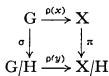
\includegraphics[keepaspectratio]{images/part002_b1d03d5a.jpg}}

于是 \(\pi \circ \rho (x) = \rho (y)\circ \sigma\)，从而

\[
\mathrm{T} _ {x} (\pi) \circ \mathrm{T} _ {e} (\rho (x)) = \mathrm{T} _ {e} (\rho (y)) \circ \mathrm{T} _ {e} (\sigma).
\]

令 \(u \in T_{e}(\mathrm{G/H})\) 满足 \(T_{e}(\rho(y))u = 0\)。存在 \(v \in T_{e}(\mathrm{G})\)，使 \(u = T_{e}(\sigma)v\)。于是 \(T_{x}(\pi)(T_{e}(\rho(x))v) = 0\)，因此 \(T_{e}(\rho(x))v\) 是 Hx 的切向量（Differentiable and Analytic Manifolds, R, 5.10.5），故其具有 \(T_{e}(\rho(x) | H)v'\) 的形式，其中 \(v' \in T_{e}(\mathrm{H})\)。由于 \(T_{e}(\rho(x))\) 是单射，所以 \(v = v'\)，从而 \(v \in T_{e}(\mathrm{H})\)，且 \(u = 0\)。因此 \(T_{e}(\rho(y))\) 是单射。\(T_{e}(\rho(y))\) 的像等于 \(T_{x}(\pi) \circ T_{e}(\rho(x))\) 的像；现在 \(T_{e}(\rho(x))\) 的像在 \(T_{x}(\mathrm{X})\) 中有拓扑补，并且包含 \(T_{x}(\pi)\) 的核。因此可见 \(\rho(y)\) 是浸入，这就完成了 (ii) 的证明。

断言 (iii) 由上述内容和 Differentiable and Analytic Manifolds, R, 5.9.7 得出。

推论。设 G 为李群，H、L 为 G 的正规李子群，且 \(L \subset H\)。则 H/L 是 G/L 的正规李子群，并且从 G/H 到 \((G/L)/(H/L)\) 的典范双射是李群同构。

